\documentclass[12pt, spanish]{article}
\usepackage[spanish]{babel}
\selectlanguage{spanish}
%\usepackage{natbib}
\usepackage{url}
\usepackage[utf8x]{inputenc}
\usepackage{graphicx}
\graphicspath{{images/}}
\usepackage{parskip}
\usepackage{fancyhdr}
\usepackage{vmargin}
\usepackage{multirow}
\usepackage{float}
\usepackage{chngpage}

\usepackage{amsfonts}

\usepackage{subcaption}

\usepackage{hyperref}
\usepackage[
    type={CC},
    modifier={by-nc-sa},
    version={4.0},
]{doclicense}

\hypersetup{
    colorlinks=true,
    linkcolor=blue,
    filecolor=magenta,
    urlcolor=cyan,
}

% para codigo
\usepackage{listings}
\usepackage{xcolor}



%% configuración de listings

\definecolor{listing-background}{HTML}{F7F7F7}
\definecolor{listing-rule}{HTML}{B3B2B3}
\definecolor{listing-numbers}{HTML}{B3B2B3}
\definecolor{listing-text-color}{HTML}{000000}
\definecolor{listing-keyword}{HTML}{435489}
\definecolor{listing-identifier}{HTML}{435489}
\definecolor{listing-string}{HTML}{00999A}
\definecolor{listing-comment}{HTML}{8E8E8E}
\definecolor{listing-javadoc-comment}{HTML}{006CA9}

\lstdefinestyle{eisvogel_listing_style}{
  language         = python,
%$if(listings-disable-line-numbers)$
%  xleftmargin      = 0.6em,
%  framexleftmargin = 0.4em,
%$else$
  numbers          = left,
  xleftmargin      = 0em,
 framexleftmargin = 0em,
%$endif$
  backgroundcolor  = \color{listing-background},
  basicstyle       = \color{listing-text-color}\small\ttfamily{}\linespread{1.15}, % print whole listing small
  breaklines       = true,
  frame            = single,
  framesep         = 0.19em,
  rulecolor        = \color{listing-rule},
  frameround       = ffff,
  tabsize          = 4,
  numberstyle      = \color{listing-numbers},
  aboveskip        = 1.0em,
  belowskip        = 0.1em,
  abovecaptionskip = 0em,
  belowcaptionskip = 1.0em,
  keywordstyle     = \color{listing-keyword}\bfseries,
  classoffset      = 0,
  sensitive        = true,
  identifierstyle  = \color{listing-identifier},
  commentstyle     = \color{listing-comment},
  morecomment      = [s][\color{listing-javadoc-comment}]{/**}{*/},
  stringstyle      = \color{listing-string},
  showstringspaces = false,
  escapeinside     = {/*@}{@*/}, % Allow LaTeX inside these special comments
  literate         =
  {á}{{\'a}}1 {é}{{\'e}}1 {í}{{\'i}}1 {ó}{{\'o}}1 {ú}{{\'u}}1
  {Á}{{\'A}}1 {É}{{\'E}}1 {Í}{{\'I}}1 {Ó}{{\'O}}1 {Ú}{{\'U}}1
  {à}{{\`a}}1 {è}{{\'e}}1 {ì}{{\`i}}1 {ò}{{\`o}}1 {ù}{{\`u}}1
  {À}{{\`A}}1 {È}{{\'E}}1 {Ì}{{\`I}}1 {Ò}{{\`O}}1 {Ù}{{\`U}}1
  {ä}{{\"a}}1 {ë}{{\"e}}1 {ï}{{\"i}}1 {ö}{{\"o}}1 {ü}{{\"u}}1
  {Ä}{{\"A}}1 {Ë}{{\"E}}1 {Ï}{{\"I}}1 {Ö}{{\"O}}1 {Ü}{{\"U}}1
  {â}{{\^a}}1 {ê}{{\^e}}1 {î}{{\^i}}1 {ô}{{\^o}}1 {û}{{\^u}}1
  {Â}{{\^A}}1 {Ê}{{\^E}}1 {Î}{{\^I}}1 {Ô}{{\^O}}1 {Û}{{\^U}}1
  {œ}{{\oe}}1 {Œ}{{\OE}}1 {æ}{{\ae}}1 {Æ}{{\AE}}1 {ß}{{\ss}}1
  {ç}{{\c c}}1 {Ç}{{\c C}}1 {ø}{{\o}}1 {å}{{\r a}}1 {Å}{{\r A}}1
  {€}{{\EUR}}1 {£}{{\pounds}}1 {«}{{\guillemotleft}}1
  {»}{{\guillemotright}}1 {ñ}{{\~n}}1 {Ñ}{{\~N}}1 {¿}{{?`}}1
  {…}{{\ldots}}1 {≥}{{>=}}1 {≤}{{<=}}1 {„}{{\glqq}}1 {“}{{\grqq}}1
  {”}{{''}}1
}
\lstset{style=eisvogel_listing_style}


\usepackage[default]{sourcesanspro}

\setmarginsrb{2 cm}{1 cm}{2 cm}{2 cm}{1 cm}{1.5 cm}{1 cm}{1.5 cm}

\title{Proyecto final:\\
Reentrenamiento de una red entrenada con\\
IMAGENET para un problema no contemplado.\hspace{0.05cm} }
\author{Juan Emilio Martínez Manjón\\
        Antonio David Villegas Yeguas}
\date{\today}

\renewcommand*\contentsname{hola}

\makeatletter
\let\thetitle\@title
\let\theauthor\@author
\let\thedate\@date
\makeatother

\pagestyle{fancy}
\fancyhf{}
\rhead{\theauthor}
\lhead{\thetitle}
\cfoot{\thepage}

\begin{document}

%%%%%%%%%%%%%%%%%%%%%%%%%%%%%%%%%%%%%%%%%%%%%%%%%%%%%%%%%%%%%%%%%%%%%%%%%%%%%%%%%%%%%%%%%

\begin{titlepage}
    \centering
    \vspace*{0.3 cm}
    
\includegraphics[scale = 0.50]{ugr.png}\\[0.7 cm]
    %\textsc{\LARGE Universidad de Granada}\\[2.0 cm]
    \textsc{\large 4º CSI 2020/21 - Grupo 2}\\[0.5 cm]
    \textsc{\large Grado en Ingeniería Informática}\\[0.5 cm]
    \rule{\linewidth}{0.2 mm} \\[0.2 cm]
    { \huge \bfseries \thetitle}\\
    \rule{\linewidth}{0.2 mm} \\[1 cm]

    \begin{minipage}{0.4\textwidth}
        \begin{flushleft} \large
            \emph{Autor:}\\
            \theauthor\\
            \end{flushleft}
            \end{minipage}~
            \begin{minipage}{0.4\textwidth}
            \begin{flushright} \large
            \emph{Asignatura: \\
            Visión por Computador}   \\
        \end{flushright}
    \end{minipage}\\[0.5cm]

    {\large \thedate}\\[0.5cm]
    %{\url{https://github.com/advy99/VC/}}
    {\doclicenseThis}

    \vfill

\end{titlepage}

%%%%%%%%%%%%%%%%%%%%%%%%%%%%%%%%%%%%%%%%%%%%%%%%%%%%%%%%%%%%%%%%%%%%%%%%%%%%%%%%%%%%%%%%%

\tableofcontents
\pagebreak

%%%%%%%%%%%%%%%%%%%%%%%%%%%%%%%%%%%%%%%%%%%%%%%%%%%%%%%%%%%%%%%%%%%%%%%%%%%%%%%%%%%%%%%%%

\section{Introducción}

De cara a desarrollar el proyecto final para la asignatura hemos decidido escoger el problema de reentrenar una red neuronal convolucional ya preentenada con un conjunto de datos (en nuestro caso ImageNet) para resolver otro problema distinto.

En concreto hemos escogido esta temática ya que nos parecía muy interesante el problema de transferencia de conocimiento de una RNN. Actualmente estamos viendo como se están desarrollando múltiples redes neuronales convolucionales que son capaces de resolver gran cantidad de problemas, sin embargo, como vimos en la práctica dos de la asignatura, es muy común el reutilizar una red para otro problema distinto al entrenado, ya sea utilizando sus parámetros si se tratan de problemas similares, reentrenando la red completa, o haciendo un fine tuning debido al coste computacional que conlleva entrenar una red neuronal convolucional desde cero. Por este motivo nos hemos interesado en estudiar más a fondo este problema, así como intentar aplicarlo a un problema que habitualmente no es muy tratado, la detección de un tipo de platos de comida concretos.


\vspace{5 mm}

\subsection{Motivación}

\vspace{5 mm}

El principal motivo por el que queremos desarrollar una CNN que reconozca platos de comida, concretamente platos de la cocina tradicional Vietnamita, es que no se trata de un campo muy explotado dentro de la clasificación de imágenes.

\vspace{3 mm}

Hay muchos papers que hablan de CNN para la clasificación de comida, donde se suele utilizar el famoso dataset \textbf{Food-101} para su entrenamiento. Estas CNN reconocen los platos de cómida más \textit{típicos} a nivel mundial, pero lo interesante y por lo que estamos haciendo este trabajo, es ver cómo podemos hacer que una CNN que reconozca estos platos \textit{típicos}, reconozca también platos tan concretos como los de la cocina Vietnamita.

\vspace{3 mm}

La Singapore Management University (SMU) desarrolló en el año 2017 una CNN llamada \textbf{foodai} capaz de reconocer 756 clases de comida entre las que había platos e ingredientes individuales. Si le pasamos a esta CNN la siguiente imagen la clasificaría sin problema como \textbf{Fried Pork Chop}:

\vspace{5 mm}

\begin{figure}[H]
  \centering
  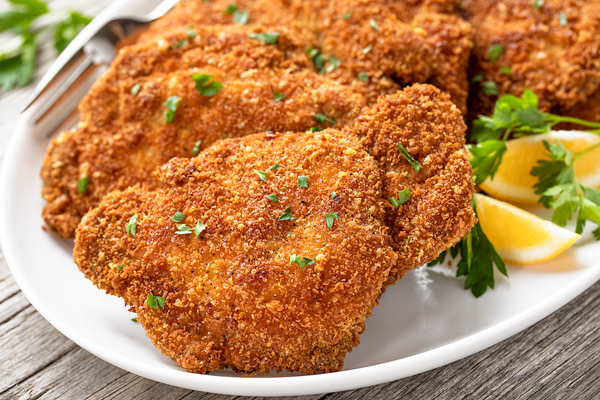
\includegraphics[width=0.5\linewidth]{Imagenes/empanada.jpeg}
  \caption{Fried Pork Chop}
  \label{fig:sub-first}
\end{figure}

Pero, ¿qué pasaría si le pasamos a la CNN un plato típico de la comida Vietnamita como puede ser el \textbf{Bun Bo Hue}?

\vspace{5 mm}

\begin{figure}[H]
  \centering
  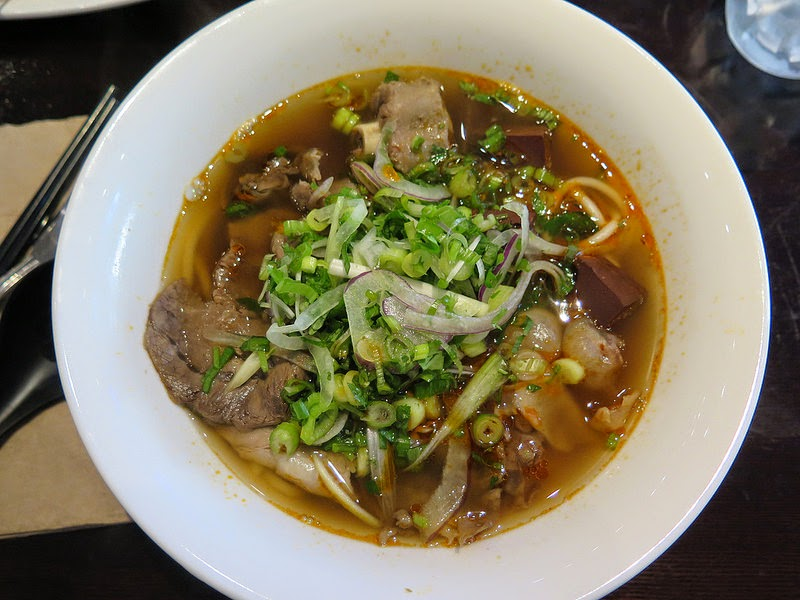
\includegraphics[width=0.5\linewidth]{Imagenes/bunbohue.jpeg}
  \caption{Bun Bo Hue}
  \label{fig:sub-first}
\end{figure}

\vspace{5 mm}

La CNN no habrá sido entrenada con la clase \textbf{Bun Bo Hue} y por lo tanto no podrá clasificar el plato correctamente, por lo que lo clasificará en una clase parecida.

\vspace{3 mm}

Es por todo lo anterior que queremos desarrollar una CNN que reconozca platos típicos de la comida Vietnamita, al igual que platos más \textit{generales} y otras clases pertenecientes al dataset \textbf{ImageNet}.

\newpage

\subsection{Pasos a seguir para conseguir nuestro objetivo}

De cara al desarrollo del proyecto comenzaremos con una introducción teórica a las redes neuronales convolucionales, tanto de su funcionamiento teórico como de la herramienta que utilizaremos para el desarrollo del proyecto, Keras. Tras la explicación de los fundamentos teóricos hablaremos del estado del arte de este problema, el cuál se ha estado desarrollando los últimos años; que se ha llegado a conseguir similar a nuestro problema, y que diferencias principales hay entre esos avances y nuestro problema concreto.

Como se nos ha recomendado, de cara a desarrollar nuestro proyecto, la base del estado del arte será fundamental ya que nos permitirá conocer que puede funcionar o no para nuestro problema concreto, además de dar un apoyo teórico y práctico más fuerte a la hora de realizar el trabajo sin tratarse simplemente de un ajuste fino como hicimos en la práctica dos de la asignatura.

Esto lo podremos llevar a cabo debido a que, aunque el problema de clasificar comida no es muy habitual, podemos encontrar algunos casos concretos en los que se ha avanzado bastante como FoodAI, o algunas redes neuronales preparadas para reconocer la base de imágenes Food101 que aunque se traten de problemas más genéricos que el nuestro nos pueden ayudar para el problema de la detección de un tipo concreto de comida.

\section{Fundamentos Teóricos}

\vspace{5 mm}

En este apartado explicaremos los principales fundamentos teóricos de las CNN's desde el punto de vista de Keras, que es la API que usaremos para desarrollar nuestro trabajo. Además, Keras es la API por excelencia para la construcción de CNN's.

\vspace{1 cm}

\subsection{¿Qué es una Red Neuronal Convolucional?}

\vspace{5 mm}

Una Red Neuronal Convolucional consiste en un conjunto de capas de filtros convolucionales de diferentes dimensiones. Estas capas son activadas por funciones de activación para dar no-linealidad a la red. Junto a estas capas se utilizan otras que aportan regularización, reducción de la dimensionalidad y aumento de la no-linealidad. El output de cada capa sirve como input de la capa a la que esté conectada. Un ejemplo de la estructura final de una CNN podría ser el siguiente:

\vspace{5 mm}

\begin{figure}[H]
  \centering
  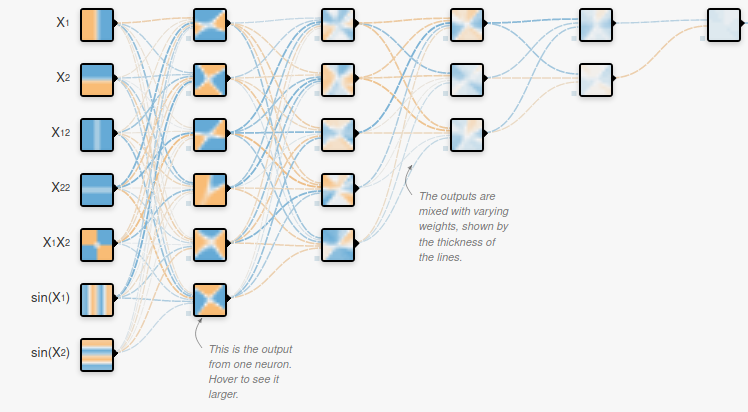
\includegraphics[width=0.5\linewidth]{Imagenes/cnn.png}
  \caption{CNN simulada en el Playground de TensorFlow}
  \label{fig:sub-first}
\end{figure}

\vspace{1 cm}

\subsection{Redes Neuronales Convolucionales para clasificación}

\vspace{5 mm}

Generalmente las Redes Neuronales Convolucionales para clasificación están formadas por capas \textbf{Conv2D}, \textbf{MaxPooling2D}, \textbf{Flatten} y \textbf{Dense}. También se usan activaciones \textbf{relu} y \textbf{softmax}. Estas capas serían las principales que toda arquitectura debería tener, pero hay muchas más.

\vspace{2 mm}

Las capas \textbf{Conv2D} producen tantas convoluciones 2D como \textbf{filters} indiquemos, usando un kernel de un tamaño \textbf{kernel\_size} que nosotros le damos. Los datos del kernel se corresponden con los pesos que ha aprendido la red neuronal hasta ese momento. La salida de una Conv2D es un bloque con tantos filtros convolucionados como indiquemos. Si no le indicamos ningún tipo de padding, las dimensiones de los filtros se verán reducidos a causa del kernel que se les pasa.

\vspace{2 mm}

Después de aplicar una capa convolucional o una capa Fully-Connected hay que aplicar una activación para modificar los valores de los filtros. Las activaciones se aplican porque en las últimas capas de nuestra red necesitamos extraer características de alto nivel que estén generalizadas para una clase particular.

\vspace{2 mm}

Por lo tanto, si no aplicasemos activaciones, los datos serían lineales y no podriamos alcanzar esa generalización que necesitamos en las últimas capas. Para darle no linealidad a los datos aplicamos dichas activaciones.

\vspace{2 mm}

Las activaciones más comunes dentro de las redes que comentaremos en posteriores apartados son las \textbf{ReLU}. Esta activación pasa los datos por la siguiente función:

\[g(z) = max(0, z)\]

De esta forma los datos negativos los convierte en 0, y los datos positivos los deja igual. Al aplicar esta función a los datos le estamos dando no linealidad a la red. Si representamos graficamente la activación obtenemos lo siguiente:

\vspace{5 mm}

\begin{figure}[H]
\centering
  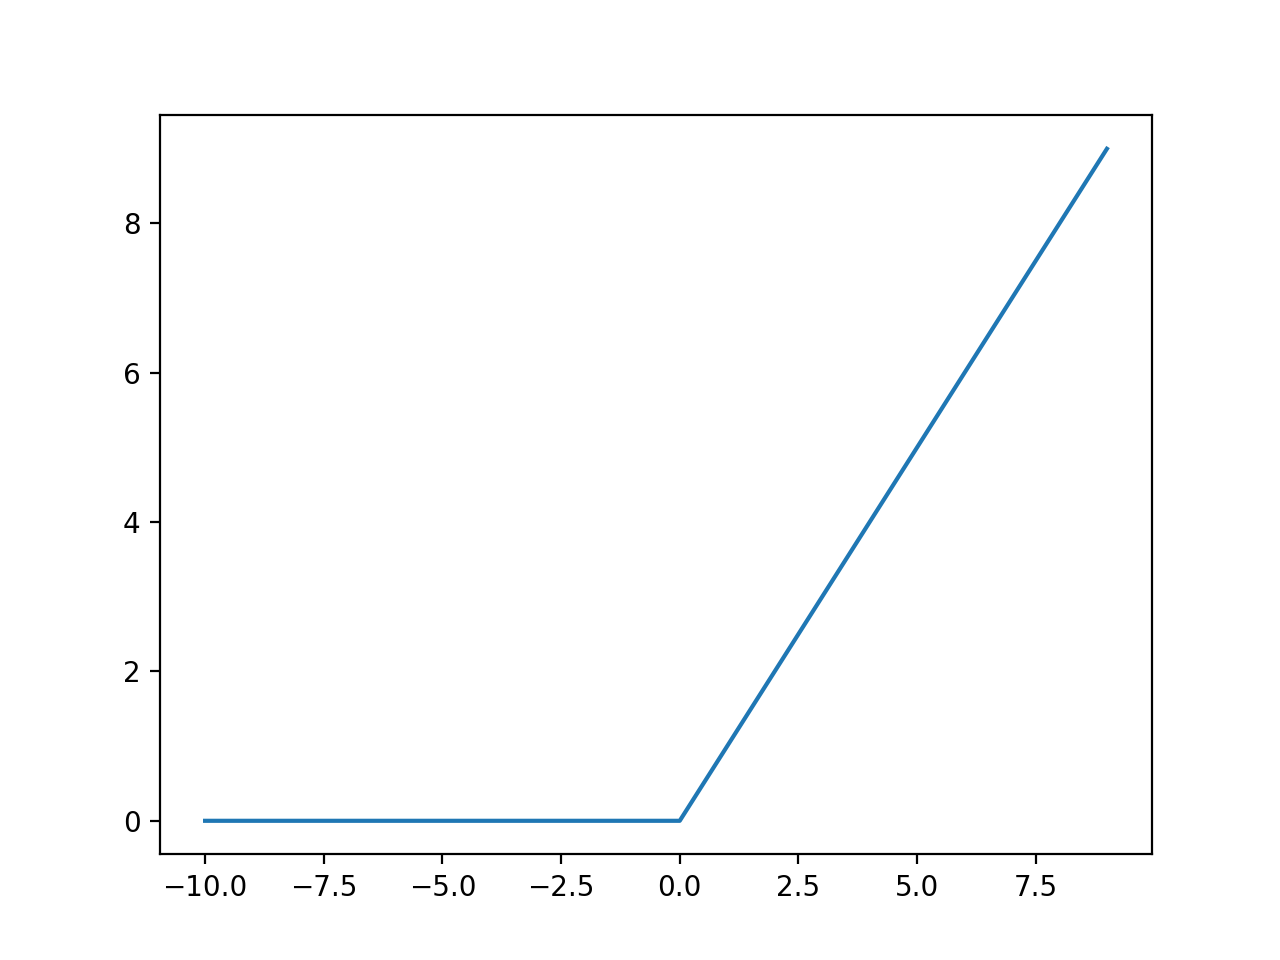
\includegraphics[width=0.5\textwidth]{Imagenes/relu.png}
   \caption{Activación Relu}
\end{figure}

\vspace{5 mm}

Vemos que los valores menores que 0 los toma directamente como 0.

\newpage

Las capas \textbf{MaxPooling2D} sirven para reducir la dimensionalidad de los filtros de tal manera que se reduce el coste computacional, también reduce la posibilidad de overfitting. Para ello utilizamos el hiperparámetro \textbf{pool\_size}. Lo que hace este valor es agrupar cada filtro en grupos de tamaño (pool\_size x pool\_size) y asignamos a cada grupo el valor máximo de los píxeles que forman el grupo. La idea se resume muy bien en la siguiente imagen:

\vspace{5 mm}

\begin{figure}[H]
\centering
  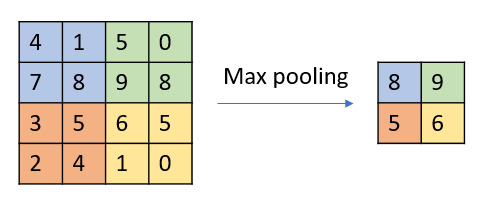
\includegraphics[width=0.5\textwidth]{Imagenes/pooling.jpg}
   \caption{MaxPooling2D de tamaño 2x2}
\end{figure}

\vspace{5 mm}

Las capas \textbf{Flatten} sirven para aplanar los bloques de filtros que tenemos hasta ese momento y convertirlos en un vector de n características. Para aplanar los filtros, lo que hace keras es multiplicar el \textbf{ancho} por el \textbf{alto} por el \textbf{numero de filtros} del que disponemos. Por ejemplo, si tuviesemos 6 filtros de 5x5, al aplicar Flatten() nos quedaríamos con un vector de 150 características.

\vspace{5 mm}

Las capas \textbf{Dense} son las conocidas como capas Fully-Connected, las cuales estan formadas por neuronas interconectadas entre si. La salida de la capa anterior se asigna a las neuronas de entrada de la capa fully-connected. A los datos que pasan por esta capa densa se les aplica una activación, en este caso \textbf{relu}, que aumenta la no linealidad del modelo. Normalmente hay menos neuronas en la salida de la capa densa que en la entrada.
La última capa de la red será otra fully-connected pero esta vez con activación \textbf{softmax}, de tal forma que tendrá tantas neuronas como clases tenga nuestra base de datos, y transformará los datos en la probabilidad de pertenecer a cada clase. La idea de las capas fully-connected se puede ver en la siguiente imagen:

\vspace{5 mm}

\begin{figure}[H]
\centering
  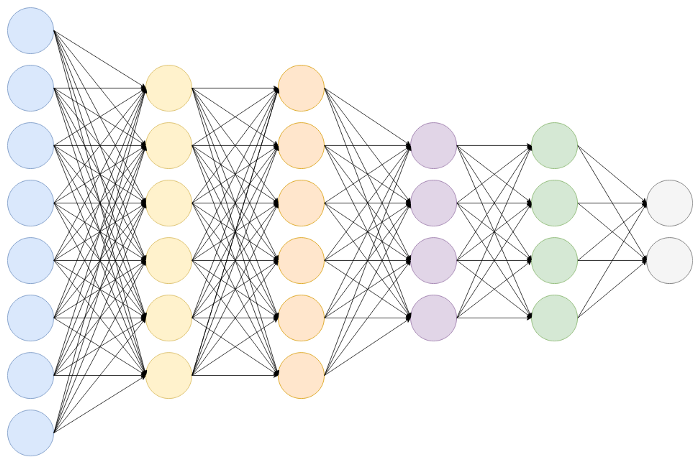
\includegraphics[width=0.5\textwidth]{Imagenes/fully.png}
   \caption{Capas Fully-Connected}
\end{figure}

\vspace{5 mm}

Una vez tenemos nuestro modelo, es necesario compilarlo usando una \textbf{función de pérdida}, un \textbf{optimizador} y una \textbf{métrica}.

\vspace{2 mm}

Como en este proyecto tenemos varias clases y cada imagen pertenece a una sola clase, vamos a usar como función de pérdida \textbf{categorical-crossentropy}. La entropía cruzada mide la distancia entre distribuciones de probabilidad y viene muy bien en nuestro caso porque la salida de nuestra red es un conjunto de probabilidades cuya suma es 1, ya que estamos usando una activación softmax en la última capa fully-connected.

\vspace{2 mm}

La función de pérdida es la siguiente:

\[Loss = - \sum_{i=1}^{output size}y_i * log (p_i) \]

Lo que hace esta función es, para cada conjunto de probabilidades de salida de nuestra red, ir sumando la multiplicacion de la etiqueta real de cada clase por la probabilidad que se ha calculado para esa clase. De tal forma que la única forma que tenemos de que la función de pérdida se quede en torno a cero, es multiplicar siempre la etiqueta correcta (1) por una probabilidad cercana a 1, ya que el logaritmo neperiano de 1 es 0. En nuestro caso estamos trabajando con una base de datos one-hot donde una sola etiqueta es correcta para cada imagen, por lo que el vector \textbf{"y"} estará lleno de 0 y solo tendrá un 1.

\vspace{2 mm}

Vamos a ejemplificar esto con tres etiquetas para que se entienda mejor. Imaginemos que tenemos las etiquetas \textbf{perro}, \textbf{gato} y \textbf{pájaro} y que al introducir en nuestra red una imagen de un perro obtenemos las probabilidades \textbf{0.8}, \textbf{0.6} y \textbf{0.1} respectivamente. Nuestro vector \textbf{"y"} sería \textbf{[1,0,0]} en este caso porque la única etiqueta correcta es \textbf{perro}.

\vspace{2 mm}

Si aplicamos la función de pérdida explicada con estos datos obtenemos que:

\[Loss = - (1*log(0.8) + 0*log(0.6) + 0*log(0.1)) = 0.22\]


\vspace{2 mm}

Esta función se va a ir actualizando cada vez que pase una imagen por nuestra red y nuestro objetivo en todo caso va a ser minimizarla, ya que cuanto mas pequeña sea, mejor va a ser nuestro modelo. El encargado de minimizar esta función va a ser el \textbf{optimizador}.

\vspace{5 mm}

El \textbf{optimizador} utiliza la función de pérdida como guía para ir actualizando los pesos de la red. De tal forma que si la función de pérdida va disminuyendo, el optimizador sabe que los pesos que está usando van por el buen camino, y, si la función de pérdida aumenta, el optimizador sabe que tiene que cambiar los pesos.

\vspace{2 mm}

En este caso vamos a utilizar el optimizador \textbf{Adam}, previamente estimado mediante GridSearchCV.

\vspace{5 mm}

Sabemos que la función que utiliza Adam para ir actualizando los pesos es la siguiente:

\[w_t = w_{t-1} - lr  \frac{m_t}{\sqrt{v_t} + e} \]

Siendo lr el \textbf{learning rate}, y mt y vt estimadores del primer y segundo \textbf{momento} del gradiente respectivamente. La \textbf{e} es un valor muy pequeño que se utiliza para no dividir nunca entre 0.

\vspace{5 mm}

Finalmente nos va a hacer falta establecer una \textbf{métrica} a la hora de compilar nuestro modelo. La métrica no va a influir en el aprendizaje, si no que va a ser una manera de que podamos ver lo bien que esta prediciendo nuestro modelo en cada etapa. La métrica que vamos a usar en este caso es la \textbf{accuracy}. Esta métrica divide el número de clases bien predichas entre el total de clases. Por lo que si nuestro modelo predice bien 180 etiquetas de las 300 etiquetas totales, diremos que tiene una accuracy del 60 porciento.
\section{Revisión bibliográfica}

El problema de clasificación de un tipo concreto de comida no es un problema muy común y por lo tanto estudiado. Como hemos visto en clase de teoría, el auge de la visión por computador se ha dado en el comienzo de la década del 2010, hace apenas diez años, con la aparición de modelos basados en redes neuronales convolucionales a pesar de que el modelo teórico de neurona y red neuronal llevan más tiempo en el ámbito de la informática. Esto ha sido en parte gracias al aumento de la capacidad de cómputo de los procesadores (tanto CPUs como procesadores gráficos) actuales.

Por este motivo, como era de esperar, en estos últimos diez años el uso de redes neuronales convolucionales se ha centrado en mejorar sus resultados con distintas técnicas vistas en teoría, mejorar los tiempos de ejecución buscando algoritmos eficientes o simplemente aumentando la potencia de cómputo, y los problemas que se han tratado de resolver son problemas más generales y en el caso de tratar algún problema específico se trata de un problema de gran interes común.

Estos motivos han llevado a que actualmente no se encuentre una gran cantidad de lecturas sobre nuestro problema concreto y las pocas que encontramos se tratan en su mayoría de comida en general sin distinguir su orgigen concreto, además de que estos experimentos comienzan a ser publicados a partir del año 2018.


En este año encontramos un trabajo de tres investigadores de la Universidad de Indonesia sobre detección de comida tradicional de Betawi en imágenes\cite{betawiFood}. En este paper se intenta detectar este tipo de comida utilizando una red ya preentrenada con otro conjunto de datos, un problema muy similar al nuestro, donde se obtienen unos resultados aceptables con una precisión de entre el 70\% y el 80\% dependiendo de la complejidad de la red utilizada.

Este es uno de los artículos que hemos encontrado donde se comienza a trabajar el problema de detección de comida, ya que como vemos en el paper citado como trabajos relacionados e introducción podemos encontrar que este trabajo surgió de una red neuronal profunda que consiguió muy buenos resultados a la hora de clasificar vehículos usando transferencia de conocimiento de una red ya preentrenada, por lo que los investigadores se interesaron en esto debido al gran impacto que conlleva el sector culinario en su país de origen.

Con respecto a la metodología aplicada en el artículo, vemos como se centran en aplicar un ajuste fino y reentrenar únicamente las últimas capas de distintos modelos basados en ResNet y DenseNet de cara a reentrenar la parte de la red que aplica la clasificación como tal y no la extracción de características, evitando tener que reentrenar toda la red completa con el coste computacional que conlleva. Vemos como esto le da unos resultados bastante buenos, siendo el peor caso la red ResNet101 con un 70\% de precisión, y el mejor caso DenseNet169 con una precisión del 80\%.


Como conclusiones de este trabajo encontramos que, si se realiza de forma correcta, el realizar un ajuste fino de una red con el nuevo conjunto de imágenes a entrenar podemos obtener un buen resultado, por lo que será lo primero que intentaremos hacer en nuestro proyecto, y a partir de ahí decidir si es necesario modificar las distintas capas de la red (ya sea añadiendo o eliminando capas), de cara a buscar unos mejores resultados.


Tras esta artículo, podemos encontrar ... (seguir con bibliografia)

\section{Metodología utilizada}


\subsection{Base de datos utilizada}

\vspace{5 mm}

A continuación hablaremos sobre la base de datos que hemos utilizado, los inconvenientes que hemos encontrado al usarla y como los hemos solucionado.

La base de datos que hemos usado se llama \textbf{Vietnamese Foods} y la subío un estudiante de la VNU HCMC a la web \textbf{kaggle}. Este dataset consta de 24474 imágenes divididas en 29 clases. Las imágenes no fueron previamente divididas en un set de entrenamiento y un set de test. Tampoco disponíamos de un archivo de texto con la ruta de todas las imágenes del dataset por lo que tuvimos que construirlo a mano usando la orden \textbf{find} que nos proporciona el terminal de Linux.

Una vez obtenido dicho archivo de texto con las imágenes nos fue sencillo construir los correspondientes sets de entrenamiento y test. Tuvimos que cargar todas las imágenes con sus respectivas clases en dos ndarrays, y usarlos en la función \textbf{train\_test\_split} de sklearn con un 0.2 de tamaño de test. Como las clases que usamos eran de tipo string, tuvimos que hacer uso también de la función \textbf{to\_categorical} para convertirlas en valores enteros.

Una vez intentamos cargar las imágenes en memoria nos dimos cuenta que no era posible debido al costo computacional que requería almacenar tantas imágenes en la RAM. Por este motivo redujimos el número de clases de forma aleatoria hasta llegar a \textbf{9}, que era el máximo número de clases que podíamos cargar en Google Colab sin sobrepasar sus recursos computacionales. Hemos decidido tomar esta decisión en lugar de reducir el número de imágenes de cada clase y mantener el número de clases ya que esto generaría una falta de datos a la hora de entrenar cada clase. Cabe destacar que todas las clases del dataset están equilibradas. A continuación mostraré ejemplos de las diferentes imágenes que se pueden encontrar en el dataset usado:

\vspace{5 mm}

\begin{figure}[H]
  \centering
  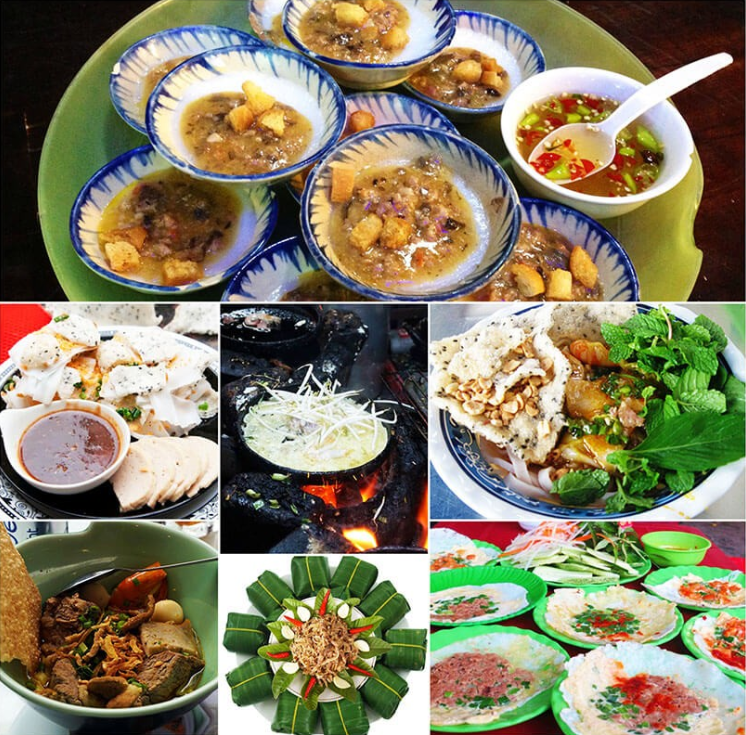
\includegraphics[width=0.5\linewidth]{Imagenes/comida-vietnamita.png}
  \caption{Imágenes del dataset Vietnamese Foods}
  \label{fig:sub-first}
\end{figure}

\newpage

\subsection{Preprocesado de los datos}

Para el preprocesado de los datos a utilizar simplemente hemos utilizado la función de preprocesado de cada red utilizada. Además de esto también hemos redimensionado las imágenes al leerlas de cara a que tengan el mismo tamaño que la entrada de las distintas redes.

También mencionar que este preprocesado se ha aplicado también al conjunto de test a la hora de predecir los valores, como vimos que es necesario tanto en teoría como en la práctica 2.


\subsection{Redes neuronales convolucionales entrenadas con ImageNet utilizadas}

\vspace{5 mm}

En el enunciado del proyecto se nos dice que usemos una red preentrenada en \textbf{ImageNet} de entre un conjunto de redes. Después de analizar los proyectos que hemos incluido en la revisión bibliográfica nos hemos dado cuenta de lo interesante que es analizar el comportamiento de cada red usando la misma base de datos. Es por todo lo anterior que hemos utilizado las siguientes redes neuronales en nuestro proyecto:

\begin{itemize}


\item{\textbf{ResNet-50:}\cite{resnet50} Esta red está compuesta por 48 capas convolucionales junto con 1 capa MaxPooling2D y 1 capa AveragePooling. Tiene un total de 25,636,712 parámetros y una media de 0.749 de Top-1 Accuracy. Se trata de una red muy útil que se usa tanto dentro como fuera de la Visión por Computador.}


\item{\textbf{EfficientNetB0:}\cite{efficientnetb0} Esta red está compuesta por 237 capas divididas en 5 tipos de módulos, donde cada uno de ellos tiene un número de capas diferentes. La red no fue desarrollada por ingenieros, si no por la propia red, la cual utiliza una búsqueda de arquitectura neuronal multiobjetivo que optimiza tanto la precisión como las operaciones de punto flotante. Tiene un total de 5,330,571 parámetros.}

\item{\textbf{DenseNet-121:}\cite{densenet121} Todas las arquitecturas DenseNet están formadas por 4 bloques densos que, dependiendo de la versión que usemos, van a tener diferentes capas en cada uno de esos bloques. Concretamente la versión DenseNet-121 va a tener 6,12,24,16 capas en cada uno de esos bloques respectivamente. Esta versión tiene un total de 8,062,504 parámetros y una media de 0.750 de Top-1 Accuracy.}


\item{\textbf{InceptionV3:}\cite{inceptionv3} Esta red tiene una profundidad de 159 capas. Está compuesta por 11 módulos Inception donde cada módulo consiste en capas MaxPooling2D y capas convolucionales con activación ReLU. Tiene un total de 23,851,784 parámetros y una media de 0.779 de Top-1 Accuracy.}


\end{itemize}

\newpage

\subsection{Mejoras sobre las redes utilizadas}

De cara a mejorar las redes utilizadas hemos realizado distintos experimentos.

Para comenzar, hemos buscado el mejor optimizador posible utilizando una Grid Search, escogiendo finalmente el optimizador Adam, explicado en los fundamentos teoricos de este documento.

Otra de las mejoras introducidas es una ampliación de las redes utilizadas, hemos añadido nuevas capas finales con el objetivo de evitar el sobreajuste de los modelos iniciales, que comentaremos en la sección de resultados, añadiendo capas de dropout y batch normalization.

\begin{lstlisting}
nueva_red = red.output
nueva_red = Dense(1000, activation="relu")(nueva_red)
nueva_red = BatchNormalization(renorm=True)(nueva_red)
nueva_red = Dropout(0.5)(nueva_red)
nueva_red = Dense (NUM_CLASES, activation = 'softmax')(nueva_red)
\end{lstlisting}

También hemos realizado un ajuste fino de la red. Hemos probado tanto a entrenar solo la última capa (capa softmax que sustituye a última capa original y que clasificará la entrada en las clases), y tras eso descongelar la red para hacer el ajuste fino tanto a entrenar las últimas cinco capas más las nuevas capas y tras eso descongelar toda la red y aplicar el ajuste fino.

Ejemplo de crear una red ResNet50 y descongelar las últimas 5 capas.

\begin{lstlisting}
#  celda para el codigo de resnet50, por defecto sin include_top para añadir la capa Dense con nuestro numero de clases y pesos de imagenet
red_resnet = ResNet50(include_top = False, pooling = "avg")
red_resnet.trainable = False
# ponemos los ultimos cinco como entrenables, el resto los fijamos
for layer in red_resnet.layers[-5:]:
  layer.trainable = True
\end{lstlisting}

Por último, y para todos los casos, hemos añadido early stopping de cara a detener el entrenamiento cuando no se logra mejorar el resultado durante cinco épocas, manteniendo los parámetros de la mejor época y no de la última.

\section{Resultados}


\subsection{Entrenando la última capa}

\subsubsection{ResNet-50}

\begin{figure}[H]
  \centering
  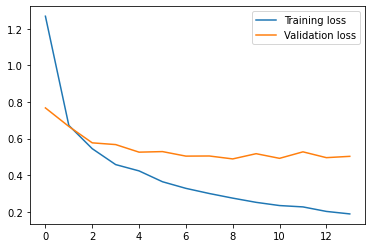
\includegraphics[width=0.5\linewidth]{Imagenes/entrenamiento_redes/ult/resnet_ult_loss.png}
  \caption{Perdida en ResNet50 entrenando unicamente la última capa.}
\end{figure}

\begin{figure}[H]
  \centering
  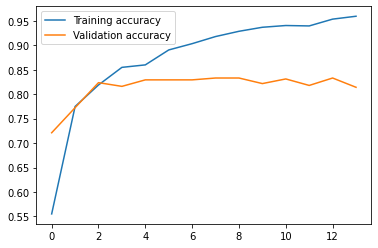
\includegraphics[width=0.5\linewidth]{Imagenes/entrenamiento_redes/ult/resnet_ult_acc.png}
  \caption{Precisión en ResNet50 entrenando unicamente la última capa.}
\end{figure}

\begin{figure}[H]
  \centering
  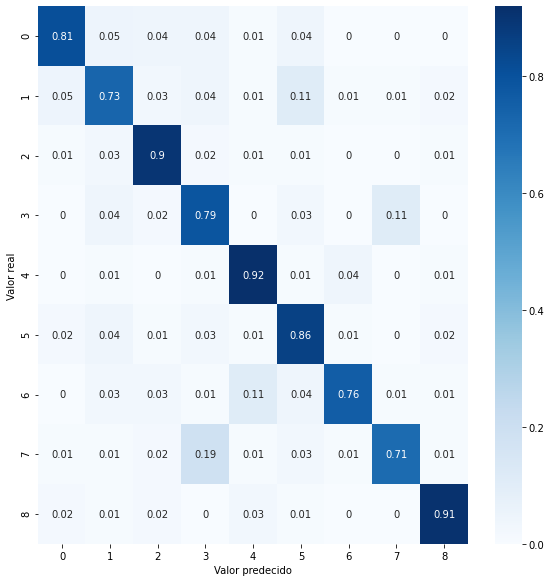
\includegraphics[width=0.5\linewidth]{Imagenes/entrenamiento_redes/ult/resnet_ult_matriz.png}
  \caption{Matriz de confusión sobre los datos de test en ResNet50 entrenando unicamente la última capa.}
\end{figure}

\begin{lstlisting}
Accuracy con ResNet50 entrenando solo ultima capa: 0.8180439727065959
\end{lstlisting}

Vemos que si entrenamos solamente la última capa de ResNet-50, congelando el resto de pesos, obtenemos una Accuracy cercana al 82$%$. Las curvas mostradas en la \textbf{Figura 16} nos dan a entender que el modelo produce un poco de overfitting y que una posible mejora puede ser aplicar técnicas de regularización al mismo. Vamos a ver qué pasa si después de entrenar la última capa, realizamos un ajuste fino de toda la red descongelando los pesos de la misma.

\begin{figure}[H]
  \centering
  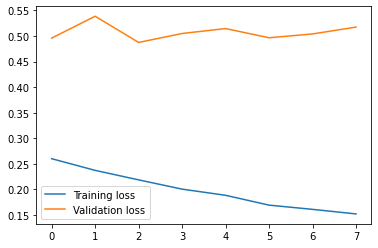
\includegraphics[width=0.5\linewidth]{Imagenes/entrenamiento_redes/ult/resnet_fine_loss.png}
  \caption{Perdida en ResNet50 entrenando unicamente la última capa y tras ajuste fino.}
\end{figure}

\begin{figure}[H]
  \centering
  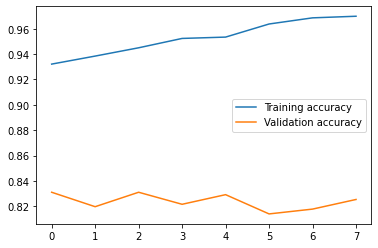
\includegraphics[width=0.5\linewidth]{Imagenes/entrenamiento_redes/ult/resnet_fine_acc.png}
  \caption{Precisión en ResNet50 entrenando unicamente la última capa y tras ajuste fino.}
\end{figure}

\begin{figure}[H]
  \centering
  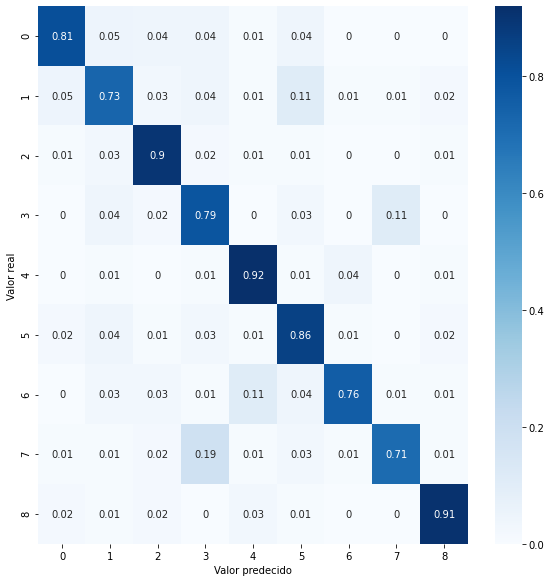
\includegraphics[width=0.5\linewidth]{Imagenes/entrenamiento_redes/ult/resnet_fine_matriz.png}
  \caption{Matriz de confusión sobre los datos de test en ResNet50 entrenando unicamente la última capa y tras ajuste fino..}
\end{figure}

\begin{lstlisting}
Accuracy con ResNet50 tras ajuste fino: 0.8180439727065959
\end{lstlisting}

Si observamos las curvas de precisión de la \textbf{Figura 19} podemos ver que al hacer el ajuste fino los resultados no mejoran. Esto lo podemos observar también al ver la Accuracy en Test, ya que es la misma que cuando hemos entrenado solamente la última capa. La Accuracy se ha mantenido porque estamos usando Early-Stopping y hemos mantenido los pesos que teníamos en vez de empeorarlos.

\subsubsection{DenseNet-121}


\begin{figure}[H]
  \centering
  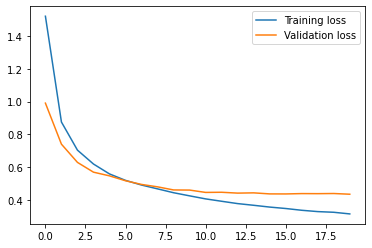
\includegraphics[width=0.5\linewidth]{Imagenes/entrenamiento_redes/ult/densenet_ult_loss.png}
  \caption{Perdida en DenseNet121 entrenando unicamente la última capa.}
\end{figure}

\begin{figure}[H]
  \centering
  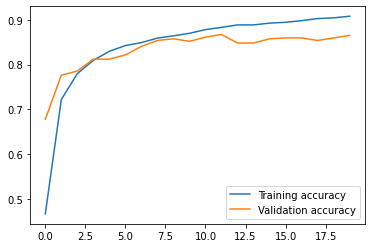
\includegraphics[width=0.5\linewidth]{Imagenes/entrenamiento_redes/ult/densenet_ult_acc.png}
  \caption{Precisión en DenseNet121 entrenando unicamente la última capa.}
\end{figure}

\begin{figure}[H]
  \centering
  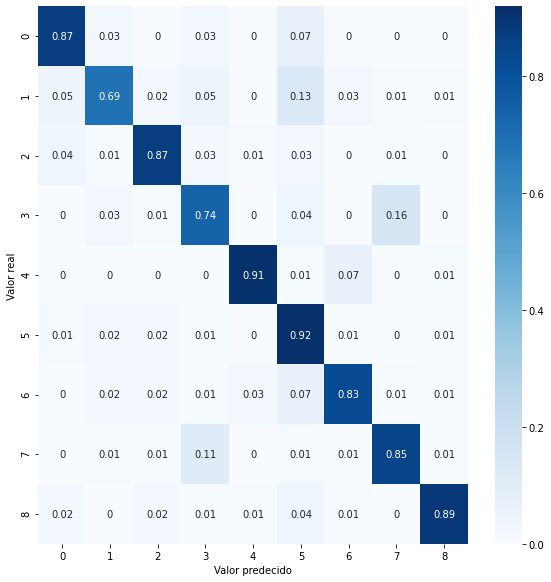
\includegraphics[width=0.5\linewidth]{Imagenes/entrenamiento_redes/ult/densenet_ult_matriz.png}
  \caption{Matriz de confusión sobre los datos de test en DenseNet121 entrenando unicamente la última capa.}
\end{figure}

\begin{lstlisting}
Accuracy con DenseNet121 entrenando solo ultima capa: 0.8377558756633814
\end{lstlisting}





\begin{figure}[H]
  \centering
  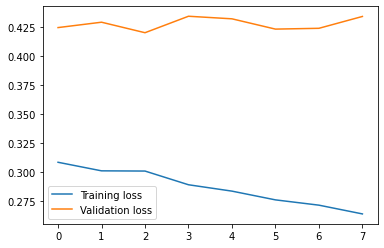
\includegraphics[width=0.5\linewidth]{Imagenes/entrenamiento_redes/ult/densenet_fine_loss.png}
  \caption{Perdida en DenseNet121 entrenando unicamente la última capa y tras ajuste fino.}
\end{figure}

\begin{figure}[H]
  \centering
  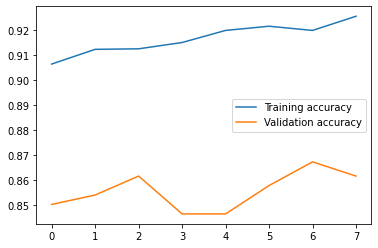
\includegraphics[width=0.5\linewidth]{Imagenes/entrenamiento_redes/ult/densenet_fine_acc.png}
  \caption{Precisión en DenseNet121 entrenando unicamente la última capa y tras ajuste fino.}
\end{figure}

\begin{figure}[H]
  \centering
  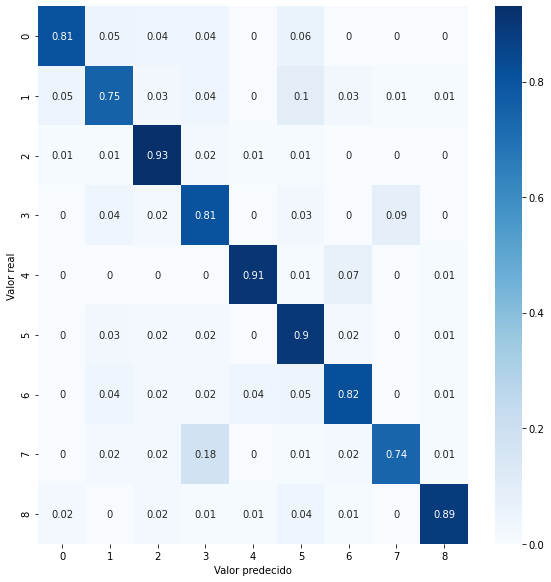
\includegraphics[width=0.5\linewidth]{Imagenes/entrenamiento_redes/ult/densenet_fine_matriz.png}
  \caption{Matriz de confusión sobre los datos de test en DenseNet121 entrenando unicamente la última capa y tras ajuste fino.}
\end{figure}


\begin{lstlisting}
Accuracy con DenseNet121 tras ajuste fino: 0.8385140257771039
\end{lstlisting}



\subsubsection{InceptionV3}

\begin{figure}[H]
  \centering
  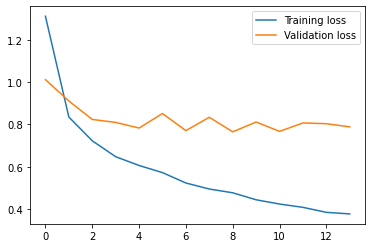
\includegraphics[width=0.5\linewidth]{Imagenes/entrenamiento_redes/ult/inception_ult_loss.png}
  \caption{Perdida en InceptionV3 entrenando unicamente la última capa.}
\end{figure}

\begin{figure}[H]
  \centering
  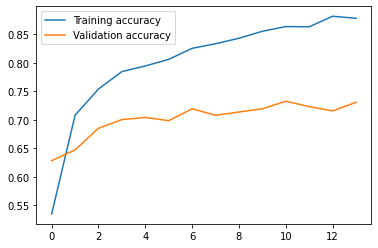
\includegraphics[width=0.5\linewidth]{Imagenes/entrenamiento_redes/ult/inception_ult_acc.png}
  \caption{Precisión en InceptionV3 entrenando unicamente la última capa.}
\end{figure}

\begin{figure}[H]
  \centering
  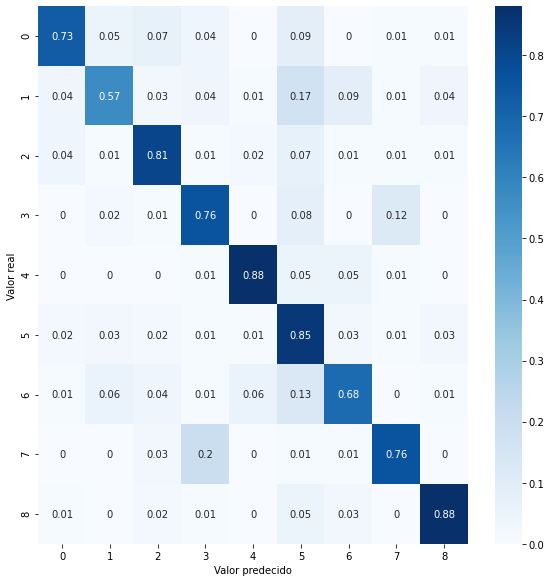
\includegraphics[width=0.5\linewidth]{Imagenes/entrenamiento_redes/ult/inception_ult_matriz.png}
  \caption{Matriz de confusión sobre los datos de test en InceptionV3 entrenando unicamente la última capa.}
\end{figure}


\begin{lstlisting}
Accuracy con InceptionV3 entrenando solo ultima capa: 0.7672479150871873
\end{lstlisting}


\begin{figure}[H]
  \centering
  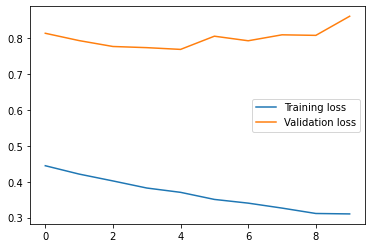
\includegraphics[width=0.5\linewidth]{Imagenes/entrenamiento_redes/ult/inception_fine_loss.png}
  \caption{Perdida en InceptionV3 entrenando unicamente la última capa y tras ajuste fino.}
\end{figure}

\begin{figure}[H]
  \centering
  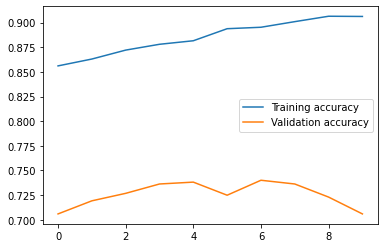
\includegraphics[width=0.5\linewidth]{Imagenes/entrenamiento_redes/ult/inception_fine_acc.png}
  \caption{Precisión en InceptionV3 entrenando unicamente la última capa y tras ajuste fino.}
\end{figure}

\begin{figure}[H]
  \centering
  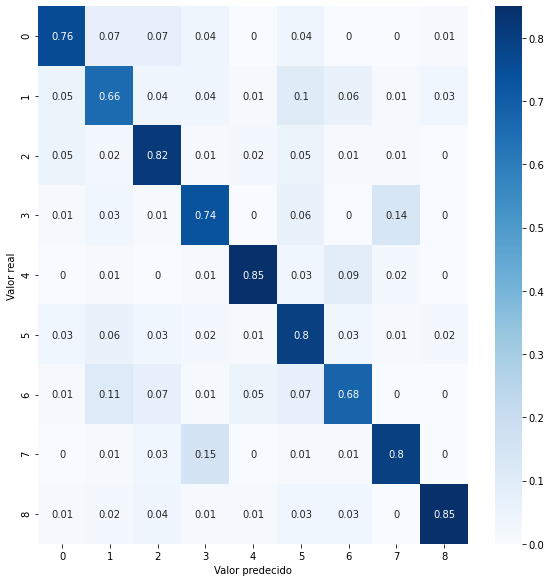
\includegraphics[width=0.5\linewidth]{Imagenes/entrenamiento_redes/ult/inception_fine_matriz.png}
  \caption{Matriz de confusión sobre los datos de test en InceptionV3 entrenando unicamente la última capa y tras ajuste fino.}
\end{figure}


\begin{lstlisting}
Accuracy con InceptionV3 tras ajuste fino: 0.7687642153146323
\end{lstlisting}


\subsubsection{EfficientNetB0}

\begin{figure}[H]
  \centering
  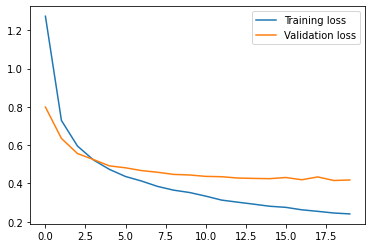
\includegraphics[width=0.5\linewidth]{Imagenes/entrenamiento_redes/ult/efficientnet_ult_loss.png}
  \caption{Perdida en EfficientNetB0 entrenando unicamente la última capa.}
\end{figure}

\begin{figure}[H]
  \centering
  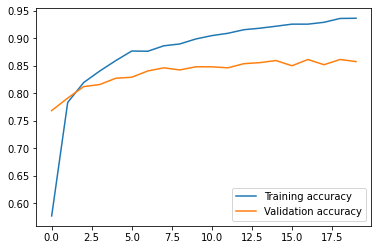
\includegraphics[width=0.5\linewidth]{Imagenes/entrenamiento_redes/ult/efficientnet_ult_acc.png}
  \caption{Precisión en EfficientNetB0 entrenando unicamente la última capa.}
\end{figure}

\begin{figure}[H]
  \centering
  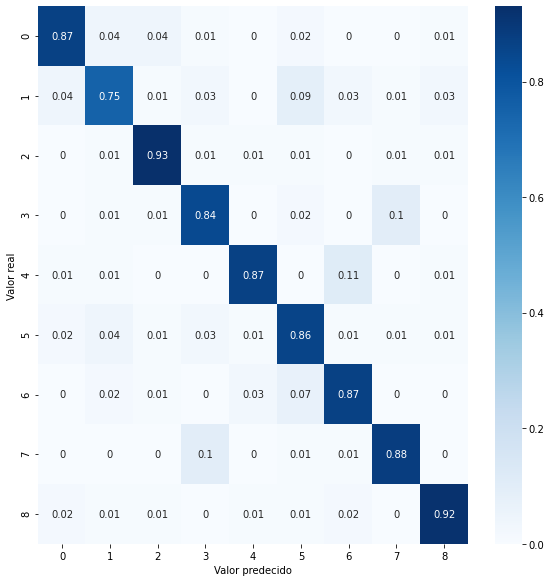
\includegraphics[width=0.5\linewidth]{Imagenes/entrenamiento_redes/ult/efficientnet_ult_matriz.png}
  \caption{Matriz de confusión sobre los datos de test en EfficientNetB0 entrenando unicamente la última capa.}
\end{figure}


\begin{lstlisting}
Accuracy con EfficientNetB0 entrenando solo ultima capa: 0.8612585291887794
\end{lstlisting}

Vemos que EfficientNetB0 comienza con una Accuracy muy alta si observamos las curvas de la \textbf{Figura 34}, llegando hasta un 86$%$ de Accuracy aproximadamente. Es uno de los resultados más altos que hemos obtenido hasta este momento entrenando solamente la capa de salida. Una posible mejora puede ser añadirle regularización a la red para que la curva de validación se mantenga más pegada a la de entrenamiento durante más tiempo. Vamos a ver qué pasa si después de entrenar la última capa, realizamos un ajuste fino de toda la red descongelando los pesos de la misma.


\begin{figure}[H]
  \centering
  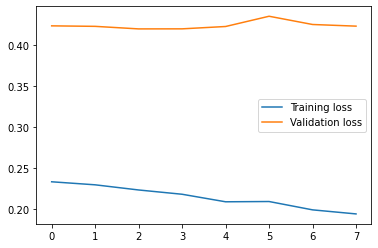
\includegraphics[width=0.5\linewidth]{Imagenes/entrenamiento_redes/ult/efficientnet_fine_loss.png}
  \caption{Perdida en EfficientNetB0 entrenando unicamente la última capa y tras ajuste fino.}
\end{figure}

\begin{figure}[H]
  \centering
  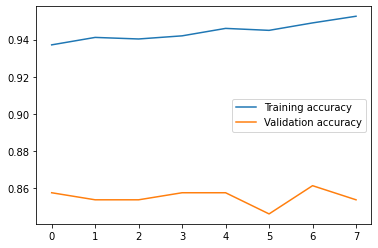
\includegraphics[width=0.5\linewidth]{Imagenes/entrenamiento_redes/ult/efficientnet_fine_acc.png}
  \caption{Precisión en EfficientNetB0 entrenando unicamente la última capa y tras ajuste fino.}
\end{figure}

\begin{figure}[H]
  \centering
  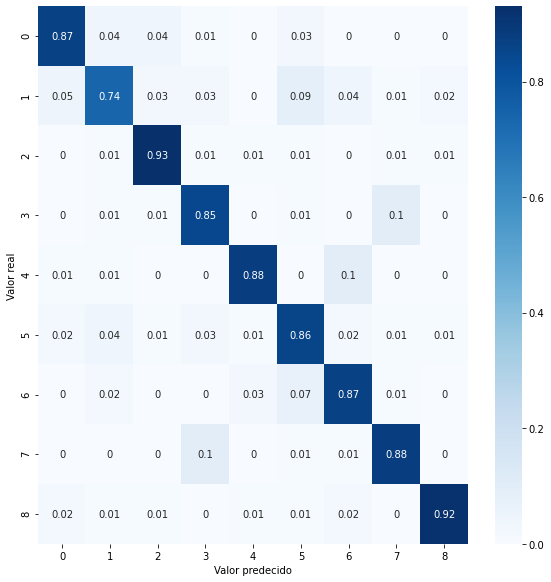
\includegraphics[width=0.5\linewidth]{Imagenes/entrenamiento_redes/ult/efficientnet_fine_matriz.png}
  \caption{Matriz de confusión sobre los datos de test en EfficientNetB0 entrenando unicamente la última capa y tras ajuste fino.}
\end{figure}

\begin{lstlisting}
Accuracy con EfficientNetB0 tras ajuste fino: 0.8627748294162244
\end{lstlisting}



Vemos que al realizar el ajuste fino pasamos de un 86.12$%$ a un 86.27$%$. No se trata de un cambio apreciable como tal pero vamos que los pesos se han ajustado un poco mejor a los datos de nuestro dataset.




% 5ult



\subsection{Entrenando las últimas cinco capas y añadiendo nuevas}

\subsubsection{ResNet-50}

\begin{figure}[H]
  \centering
  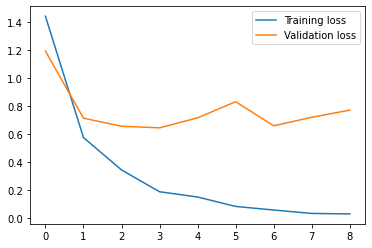
\includegraphics[width=0.5\linewidth]{Imagenes/entrenamiento_redes/5-ult/resnet_5ult_loss.png}
  \caption{Perdida en ResNet50 entrenando las cinco últimas capas y nuevas capas.}
\end{figure}

\begin{figure}[H]
  \centering
  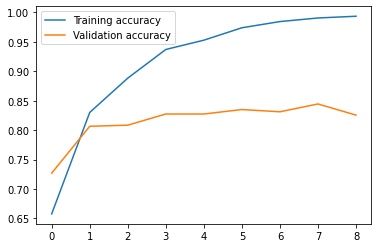
\includegraphics[width=0.5\linewidth]{Imagenes/entrenamiento_redes/5-ult/resnet_5ult_acc.png}
  \caption{Precisión en ResNet50 entrenando las cinco últimas capas y nuevas capas.}
\end{figure}

\begin{figure}[H]
  \centering
  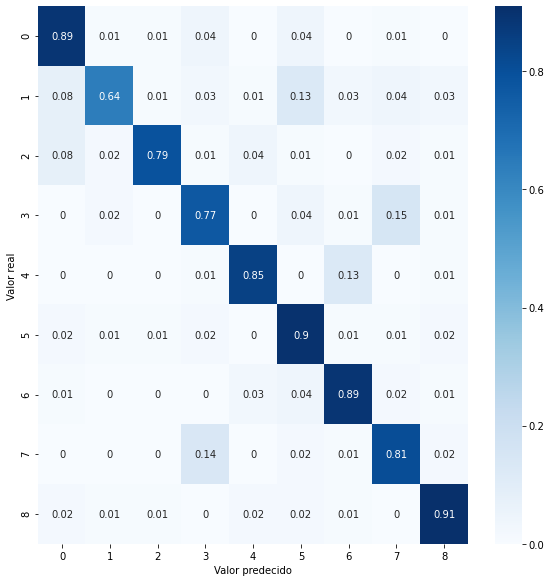
\includegraphics[width=0.5\linewidth]{Imagenes/entrenamiento_redes/5-ult/resnet_5ult_matriz.png}
  \caption{Matriz de confusión sobre los datos de test en ResNet50 entrenando las cinco últimas capas y nuevas capas.}
\end{figure}

\begin{lstlisting}
Accuracy con ResNet50 entrenando las cinco últimas capas: 0.821076573161486
\end{lstlisting}


Al entrenar las cinco últimas capas en vez de solamente la última, y añadir nuevas capas Dense, BatchNormalization y Dropout; obtenemos una accuracy del 82$%$ aproximadamente. Si miramos la Accuracy que obtuvimos cuando solo entrenamos la última capa, podemos apreciar una pequeña mejora. Vamos a ver que pasa si ahora hacemos un ajuste fino con estos nuevos pesos de las últimas capas.

\begin{figure}[H]
  \centering
  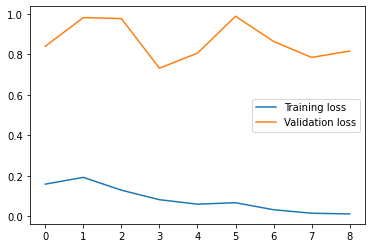
\includegraphics[width=0.5\linewidth]{Imagenes/entrenamiento_redes/5-ult/resnet_5fine_loss.png}
  \caption{Perdida en ResNet50 entrenando las cinco últimas capas y nuevas capas tras ajuste fino.}
\end{figure}

\begin{figure}[H]
  \centering
  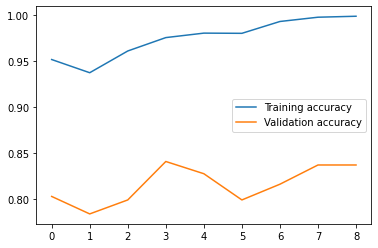
\includegraphics[width=0.5\linewidth]{Imagenes/entrenamiento_redes/5-ult/resnet_5fine_acc.png}
  \caption{Precisión en ResNet50 entrenando las cinco últimas capas y nuevas capas tras ajuste fino.}
\end{figure}

\begin{figure}[H]
  \centering
  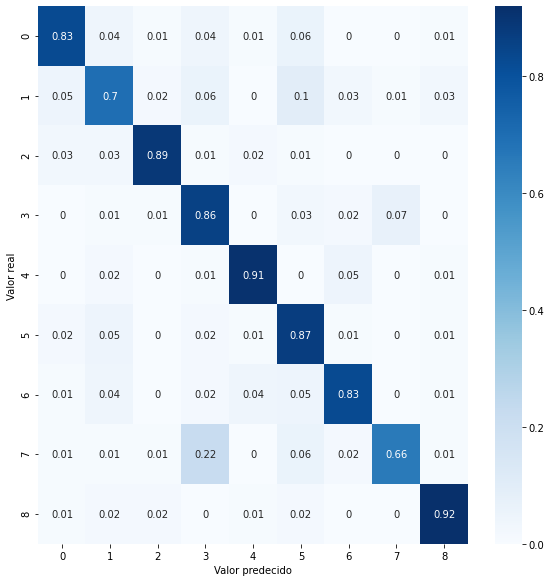
\includegraphics[width=0.5\linewidth]{Imagenes/entrenamiento_redes/5-ult/resnet_5fine_matriz.png}
  \caption{Matriz de confusión sobre los datos de test en ResNet50 entrenando las cinco últimas capas y nuevas capas tras ajuste fino..}
\end{figure}


\begin{lstlisting}
Accuracy con ResNet50 tras ajuste fino: 0.8256254738438211
\end{lstlisting}


Vemos que hemos mejorado un poco más, pasando de un 82.1$%$ a un 82.56$%$. No se trata de una mejora apreciable, como el resto de las mejoras que hemos observado, pero sabemos que estamos yendo por el camino correcto.

\subsubsection{DenseNet-121}

\begin{figure}[H]
  \centering
  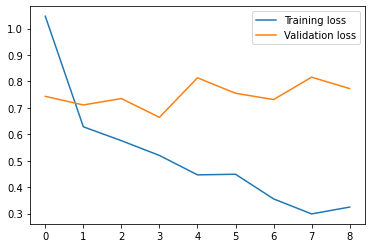
\includegraphics[width=0.5\linewidth]{Imagenes/entrenamiento_redes/5-ult/densenet_5ult_loss.png}
  \caption{Perdida en DenseNet121 entrenando las cinco últimas capas y nuevas capas.}
\end{figure}

\begin{figure}[H]
  \centering
  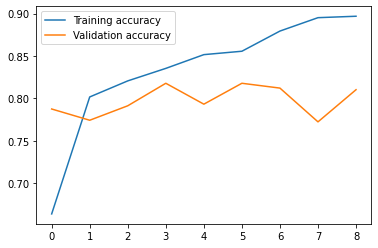
\includegraphics[width=0.5\linewidth]{Imagenes/entrenamiento_redes/5-ult/densenet_5ult_acc.png}
  \caption{Precisión en DenseNet121 entrenando las cinco últimas capas y nuevas capas.}
\end{figure}

\begin{figure}[H]
  \centering
  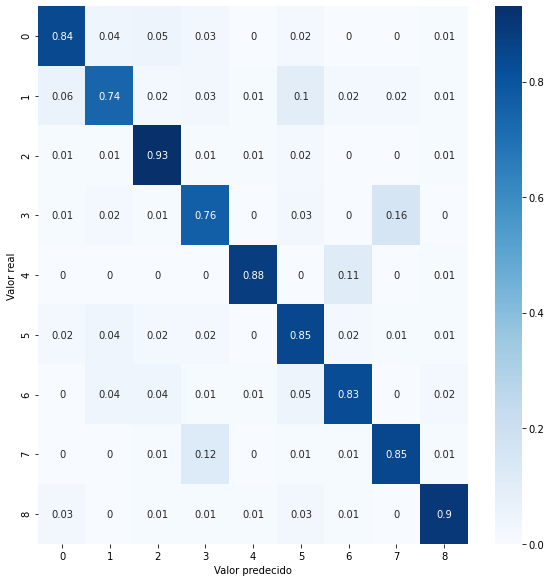
\includegraphics[width=0.5\linewidth]{Imagenes/entrenamiento_redes/5-ult/densenet_5ult_matriz.png}
  \caption{Matriz de confusión sobre los datos de test en DenseNet121 entrenando las cinco últimas capas y nuevas capas.}
\end{figure}


\begin{lstlisting}
Accuracy con DenseNet121 entrenando las ultimas 5 capas: 0.8339651250947687
\end{lstlisting}



\begin{figure}[H]
  \centering
  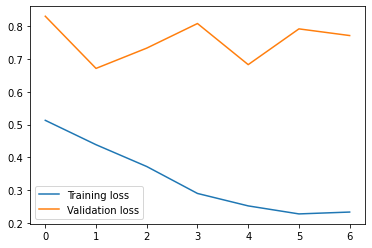
\includegraphics[width=0.5\linewidth]{Imagenes/entrenamiento_redes/5-ult/densenet_5fine_loss.png}
  \caption{Perdida en DenseNet121 entrenando las cinco últimas capas y nuevas capas tras ajuste fino.}
\end{figure}

\begin{figure}[H]
  \centering
  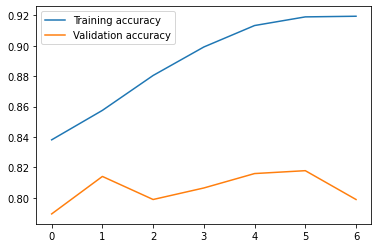
\includegraphics[width=0.5\linewidth]{Imagenes/entrenamiento_redes/5-ult/densenet_5fine_acc.png}
  \caption{Precisión en DenseNet121 entrenando las cinco últimas capas y nuevas capas tras ajuste fino.}
\end{figure}

\begin{figure}[H]
  \centering
  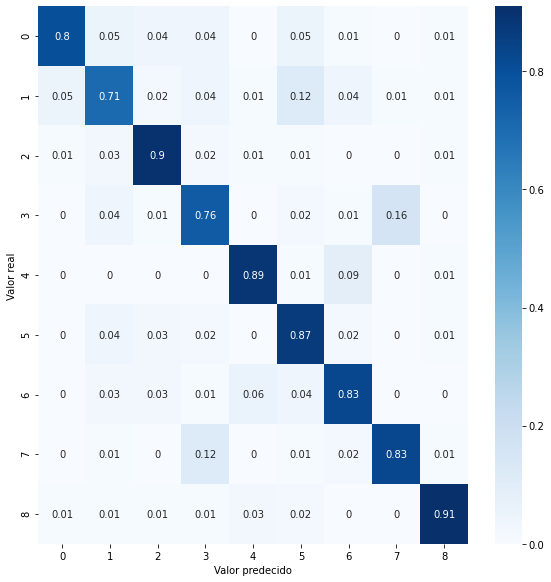
\includegraphics[width=0.5\linewidth]{Imagenes/entrenamiento_redes/5-ult/densenet_5fine_matriz.png}
  \caption{Matriz de confusión sobre los datos de test en DenseNet121 entrenando las cinco últimas capas y nuevas capas tras ajuste fino.}
\end{figure}

\begin{lstlisting}
Accuracy con DenseNet121 tras ajuste fino: 0.8263836239575436
\end{lstlisting}



\subsubsection{InceptionV3}


\begin{figure}[H]
  \centering
  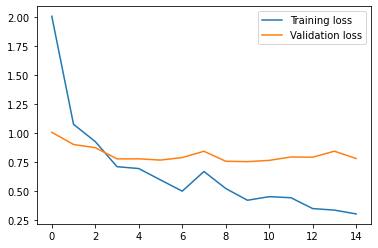
\includegraphics[width=0.5\linewidth]{Imagenes/entrenamiento_redes/5-ult/inception_5ult_loss.png}
  \caption{Perdida en InceptionV3 entrenando las cinco últimas capas y nuevas capas.}
\end{figure}

\begin{figure}[H]
  \centering
  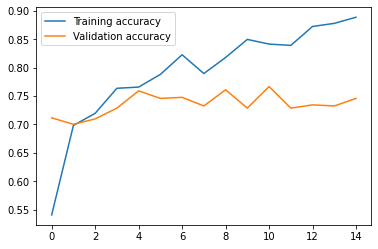
\includegraphics[width=0.5\linewidth]{Imagenes/entrenamiento_redes/5-ult/inception_5ult_acc.png}
  \caption{Precisión en InceptionV3 entrenando las cinco últimas capas y nuevas capas.}
\end{figure}

\begin{figure}[H]
  \centering
  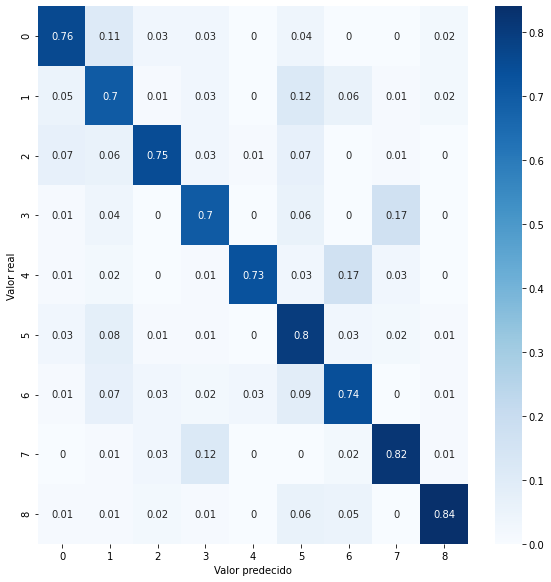
\includegraphics[width=0.5\linewidth]{Imagenes/entrenamiento_redes/5-ult/inception_5ult_matriz.png}
  \caption{Matriz de confusión sobre los datos de test en InceptionV3 entrenando las cinco últimas capas y nuevas capas.}
\end{figure}


\begin{lstlisting}
Accuracy con InceptionV3 entrenando las cinco últimas capas: 0.7589082638362395
\end{lstlisting}


\begin{figure}[H]
  \centering
  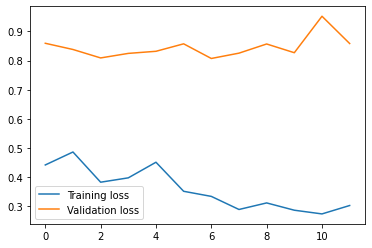
\includegraphics[width=0.5\linewidth]{Imagenes/entrenamiento_redes/5-ult/inception_5fine_loss.png}
  \caption{Perdida en InceptionV3 entrenando las cinco últimas capas y nuevas capas tras ajuste fino.}
\end{figure}

\begin{figure}[H]
  \centering
  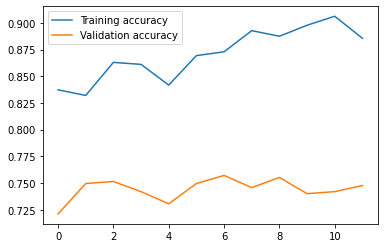
\includegraphics[width=0.5\linewidth]{Imagenes/entrenamiento_redes/5-ult/inception_5fine_acc.png}
  \caption{Precisión en InceptionV3 entrenando las cinco últimas capas y nuevas capas tras ajuste fino.}
\end{figure}

\begin{figure}[H]
  \centering
  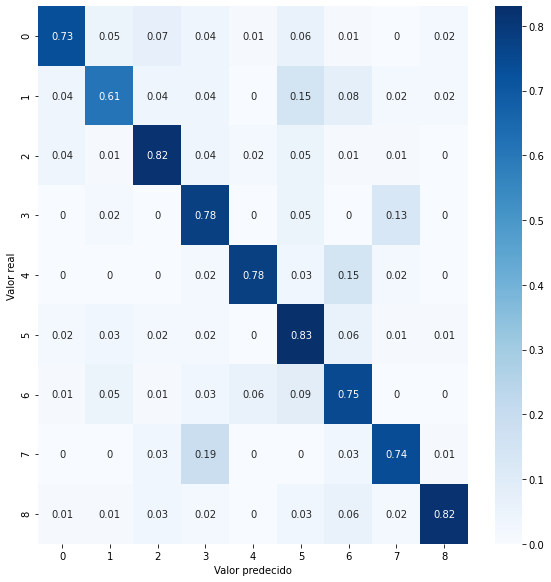
\includegraphics[width=0.5\linewidth]{Imagenes/entrenamiento_redes/5-ult/inception_5fine_matriz.png}
  \caption{Matriz de confusión sobre los datos de test en InceptionV3 entrenando las cinco últimas capas y nuevas capas tras ajuste fino.}
\end{figure}


\begin{lstlisting}
Accuracy con InceptionV3 tras ajuste fino: 0.7649734647460197
\end{lstlisting}



\subsubsection{EfficientNetB0}


\begin{figure}[H]
  \centering
  \includegraphics[width=0.5\linewidth]{Imagenes/entrenamiento_redes/5-ult/efficientnet_5ult_loss.png}
  \caption{Perdida en EfficientNetB0 entrenando las cinco últimas capas y nuevas capas.}
\end{figure}

\begin{figure}[H]
  \centering
  \includegraphics[width=0.5\linewidth]{Imagenes/entrenamiento_redes/5-ult/efficientnet_5ult_acc.png}
  \caption{Precisión en EfficientNetB0 entrenando las cinco últimas capas y nuevas capas.}
\end{figure}

\begin{figure}[H]
  \centering
  \includegraphics[width=0.5\linewidth]{Imagenes/entrenamiento_redes/5-ult/efficientnet_5ult_matriz.png}
  \caption{Matriz de confusión sobre los datos de test en EfficientNetB0 entrenando las cinco últimas capas y nuevas capas.}
\end{figure}


\begin{lstlisting}
Accuracy con EfficientNetB0 entrenando las cinco últimas capas: 0.8597422289613343
\end{lstlisting}


Al añadir más capas y entrenar las últimas cinco podemos ver que se produce mucho más overfitting que cuando solo entrenamos la última capa (Figuras 34 y 58). Incluso la Accuracy en Test ha bajado de un 86.12$%$ a un 85.9$%$. Esta decisión ha perjudicado un poco el rendimiento de la red EfficientNetB0. Vamos a ver si al realizar Fine Tuning mejoramos o seguimos empeorando.

\begin{figure}[H]
  \centering
  \includegraphics[width=0.5\linewidth]{Imagenes/entrenamiento_redes/5-ult/efficientnet_5fine_loss.png}
  \caption{Perdida en EfficientNetB0 entrenando las cinco últimas capas y nuevas capas tras ajuste fino.}
\end{figure}

\begin{figure}[H]
  \centering
  \includegraphics[width=0.5\linewidth]{Imagenes/entrenamiento_redes/5-ult/efficientnet_5fine_acc.png}
  \caption{Precisión en EfficientNetB0 entrenando las cinco últimas capas y nuevas capas tras ajuste fino.}
\end{figure}

\begin{figure}[H]
  \centering
  \includegraphics[width=0.5\linewidth]{Imagenes/entrenamiento_redes/5-ult/efficientnet_5fine_matriz.png}
  \caption{Matriz de confusión sobre los datos de test en EfficientNetB0 entrenando las cinco últimas capas y nuevas capas tras ajuste fino.}
\end{figure}


\begin{lstlisting}
Accuracy con EfficientNetB0 tras ajuste fino: 0.8567096285064443
\end{lstlisting}


Como vemos, al realizar Fine Tuning seguimos empeorando, lo que nos lleva a asegurar que las capas elegidas y descongeladas no han sido las más adecuadas para mejorar el rendimiento de la red.
\section{Conclusiones y posibles mejoras a aplicar}

\subsection{Mejor modelo para nuestro problema}

Después de realizar todas las pruebas de la sección anterior podemos concluir que el modelo preentrenado en \textbf{ImageNet} que mejor funciona con nuestro dataset es \textbf{EfficientNetB0} tras realizar un Ajuste Fino entrenando previamente la última capa solamente. Este modelo llega a alcanzar un \textbf{0.8627748294162244} de Accuracy. Hay que comentar que si hubiésemos usado una de las últimas versiones de EfficientNet, por ejemplo la B7, posiblemente la Accuracy hubiese sido mejor. No hemos podido hacer la prueba empírica debido al coste computacional que conlleva cargar un modelo con tantos parámetros, pero lo apuntamos como posible mejora.

\subsection{Transferencia de conocimiento de ImageNet}

Tras todas las pruebas y experimentos vemos como el conjunto de nuevas imágenes ha obtenido muy buenos resultados y esto es gracias a los pesos heredados de ImageNet. Como hemos visto en teoría, el conjunto de ImageNet cuenta con mil clases distintas, muchas de ellas ya pertenecientes a comida que aunque no sea en concreto nuestro problema ni sea similar como vimos en la revisión bibliográfica, hemos conseguido alcanzar muy buenos resultados reentrenando estas redes para este problema.

Como conclusión podemos obtener que este paso es muy importante y de gran ayuda en el entrenamiento debido a la gran variedad de clases con las que está entrenado ImageNet, permitiendo que gran cantidad de problemas que podamos encontrar tengan cierta similutud con alguna de las clases de ImageNet.


\subsection{Fallos comunes entre los modelos utilizados}

Al analizar las matrices de confusión nos hemos dado cuenta de que es común para todos los modelos confundir la clase 3 con la clase 7 y viceversa. 

\subsection{Posibles soluciones a estos fallos y futuras mejoras}



\newpage

\section{Referencias, material y documentación usada}

\begin{thebibliography}{9}


\end{thebibliography}

\end{document}
